\chapter{Companies and Financial Accounting}
\section{Companies}
\subsection{What is a company?}
A company is a legal entity (``personality'') that can issue contracts, enter into agreements or contracts, assume obligations, incur and pay debts, sue and be sued in its own right, and be held responsible for its own actions. There are three main types of companies in the UK:
\begin{enumerate}
    \item A Sole Trader
    \item A Partnership
    \item A Limited Liability Company
\end{enumerate}
\subsubsection{Sole Trader}
A sole Trader:
\begin{itemize}
    \item Runs their own business as an individual
    \item Keeps all of the net profits
    \item Is personally responsible for any losses their business makes (unlimited liability)
\end{itemize}
\subsubsection{Partnership}
A Partnership:
\begin{itemize}
    \item Involves two or more partners who share responsibility for the business
    \item Keeps all of the net profits (jointly)
    \item Is jointly responsible for any losses their business makes (joint unlimited liability)
    \item A partner does not have to be an actual person. For example, a limited company counts as a `legal person' and can also be a partner
\end{itemize}
\subsubsection{Limited Liability Company}
A Limited Liability Company that is ``limited by shares'' or ``limited by guarantee.''

Limited by shares:
\begin{itemize}
    \item Usually businesses that make a profit
          \begin{itemize}
              \item is legally separate from those who run it (limited liability)
              \item has shares and shareholders
              \item retains net profits
          \end{itemize}
\end{itemize}

Limited by guarantee:
\begin{itemize}
    \item Usually businesses that are ``not for profit''
          \begin{itemize}
              \item is legally separate from those who run it (limited liability)
              \item has guarantors and a ``guaranteed amount''
              \item invests profits it makes back into the company
          \end{itemize}
\end{itemize}
\subsection{Structure of a Limited Liability Company limited by shares}
\begin{figure}[H]
    \centering
    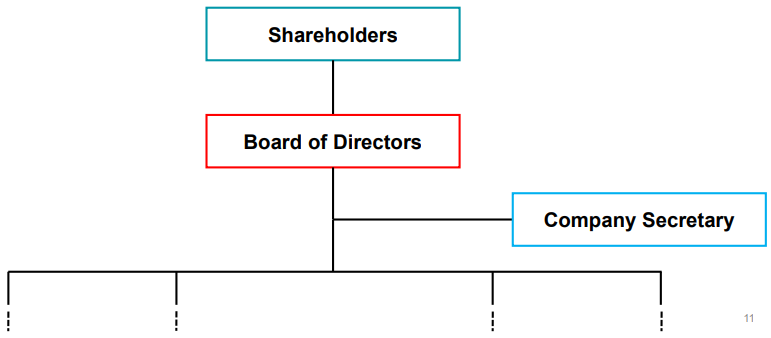
\includegraphics[width = \textwidth]{./img/figure26.png}
    \caption{Structure of a Limited Liability Company limited by shares.}
\end{figure}
\subsection{What is a shareholder?}
\begin{itemize}
    \item Shareholders own a Limited Liability Company limited by shares
    \item They have no day-to-day duties related to the company's operation
    \item Each shareholder owns a fraction of the company (and has corresponding voting power) proportional to their shareholding (investment)
    \item The liability of shareholders is limited to their original investment
    \item The company's profits are paid to shareholders as share dividend
\end{itemize}
\subsection{What is the Board of Directors?}
\begin{itemize}
    \item The Board of Directors is elected by the shareholders at the Annual General Meeting (AGM) to run the company.
          \begin{itemize}
              \item Directors may also be shareholders (but not necessarily)
              \item The shareholders can vote to appoint or sack individual Board of Directors members
          \end{itemize}
    \item The Board of Directors files the company's audited accounts (legal requirement)
    \item The Board of Directors report to the shareholders at the AGM (legal requirement)
    \item The Board of Directors is controller by the Chairman of the Board
    \item The Board of Directors can appoint or sack the Chief Executive Officer (CEO - responsible for day-to-day running)
\end{itemize}
\subsection{What is a company secretary?}
The company secretary ensures the smooth administration of the company. The company secretary is responsible for:
\begin{itemize}
    \item Making sure the company stays within the law
    \item Making sure the company maintains proper record books and accounts
    \item Providing strategic advice to the Board of Directors (sometimes)
\end{itemize}
The company secretary may or may not be a member of the Board of Directors.
\subsection{Limited Liability Company}
A Limited Liability Company that is ``limited by shares'' can be public or private.

Private Limited Company (Ltd.):
\begin{itemize}
    \item Share ownership is controlled
          \begin{itemize}
              \item is owned privately
              \item only one director is required
              \item have nine months to file their annual accounts
              \item a company secretary is not legally required
          \end{itemize}
\end{itemize}

Public Limited Company (PLC):
\begin{itemize}
    \item Share ownership is NOT controlled
          \begin{itemize}
              \item company shares can be bought and sold publically on the open market (a stock exchange)
              \item two directors are required
              \item have six months to file their annual accounts
              \item a company secretary is legally required
          \end{itemize}
\end{itemize}
\section{What is accounting?}
Accounting is the collection, analysis and communication of financial information that is used by:
\begin{itemize}
    \item Those who need to make decisions and plans in an organisation
    \item Those who need to control an organisation
\end{itemize}
Accounting helps companies to plan for the future and evaluate past performance. Accounting os often referred to as the language of business.
\section{The fundamental accounting equation}
\begin{gather}
    \textrm{Assets} = \textrm{Liabilities} + \textrm{Owners' Equity}
\end{gather}
where:
\begin{itemize}
    \item Assets are resources that a company owns. They have the capacity to provide future services or benefits. Companies use their assets in carrying out activities like production and sales
    \item Liabilities are claims against assets - existing debts and obligations. They arise from purchasing items on credit or borrowing money from a bank for purchases
    \item Owners' Equity is what remains of the assets after all liabilities have been paid
\end{itemize}
``Liabilities + Owners' Equity'' are the rights or claims against the resources of the company.
\subsection{Some important definitions}
\textbf{Assets:}
\begin{quoting}
    Economic resources that a company expects to help generate future cash inflows or help reduce future cash outflow.
\end{quoting}
\textbf{Current assets:}
\begin{quoting}
    A company's cash and other assets that are expected to be converted to cash over the next one year period.
\end{quoting}
\textbf{Non-current assets:}
\begin{quoting}
    A company's assets that are not expected to be converted to cash over the next one year period.
\end{quoting}
\textbf{Inventory:}
\begin{quoting}
    Goods (current assets) available for sale or raw materials and components used to produce goods available for sale.
\end{quoting}
\textbf{Liabilities:}
\begin{quoting}
    Economic obligations of the organisation to outsiders, or claims against its assets by outsiders.
\end{quoting}
\textbf{Current liabilities:}
\begin{quoting}
    A company's short term obligations, due within one year period.
\end{quoting}
\textbf{Non-current liabilities:}
\begin{quoting}
    A company's long-term obligations listed on the balance sheet.
\end{quoting}
\textbf{Dividends:}
\begin{quoting}
    Money paid regularly to shareholders by the company.
\end{quoting}
\section{Balance sheet}
The balance sheet is one of the two most common accounting statements. The fundamental accounting equation defines the format of the balance sheet. The balance sheet shows the financial position of the company at one instant in time (e.g. end of the quarter or end of the year).
\begin{table}[H]
    \centering
    \begin{tabular}{@{}llll@{}}
        \toprule
        Assets              &               & Liabilities / Owners' Equity &               \\
        \midrule
        Cash                & \pounds 2,500 & Accounts payable             & \pounds 1,200 \\
        Land                & \pounds 1,800 & Bank note                    & \pounds 900   \\
        Accounts receivable & \pounds 800   & Owners' Equity               & \pounds 3,000 \\
        \midrule
        Total assets        & \pounds 5,100 & Total liabilities and        & \pounds 5,100 \\
                            &               & Owners' Equity               &               \\
        \bottomrule
    \end{tabular}
    \caption{Balance sheet.}
\end{table}
\begin{gather}
    \textrm{Assets} = \textrm{Liabilities} + \textrm{Owners' Equity} = \pounds 5100
\end{gather}
\section{Income statement}
The income statement is the second of the two most common accounting statements. The income statement summarises the revenue and expense results of operations over a period of time (a moving picture.) It is defined by the following equation:
\begin{gather}
    \textrm{Profit (or Loss)} = \textrm{Revenues} - \textrm{Expenses}
\end{gather}
\begin{table}[H]
    \centering
    \begin{tabular}{@{}llll@{}}
        \toprule
        \textbf{Revenue}    &                &               &               \\
        Sales               &                &               & \pounds 3,000 \\
        \midrule
        \textbf{Expenses}   &                &               &               \\
        Labour              &                & \pounds 1,200 &               \\
        Depreciation        &                & \pounds 400   &               \\
        Material            &                & \pounds 500   &               \\
        \midrule
                            & Total Expenses &               & \pounds 2,100 \\
        \textbf{Net income} &                &               & \pounds 900   \\
        \bottomrule
    \end{tabular}
    \caption{Income statement.}
\end{table}
\subsection{Some important definitions}
\textbf{Turnover:}
\begin{quoting}
    The net sales generated by a business.
\end{quoting}
Turnover and profit are the beginning and end points of the income statement.
\section{Worked example}
John Deere owns and operates a design company called Deere Consulting Ltd. The financial position of his business is:
\begin{table}[H]
    \centering
    \begin{tabular}[]{@{}ll@{}}
        \toprule
        Cash                & \pounds 1,720  \\
        Accounts receivable & \pounds 3,240  \\
        Land                & \pounds 24,100 \\
        Accounts payable    & \pounds 5,400  \\
        John Deere, Capital & \pounds 23,660 \\
        \bottomrule
    \end{tabular}
    \caption{Financial position of John Deere Ltd.}
\end{table}
During May 2021, the following events occurred:
\begin{enumerate}
    \item Deere received \pounds 12,000 as a gift and deposited the cash in the business bank account
    \item Deere paid of the beginning balance of the accounts payable
    \item Deere performed services for a client and received cash of \pounds 1,100
    \item Deere collected \pounds 750 cash from a customer on account
    \item Deere purchased \pounds 720 of supplies on account
    \item Deere billed a client \pounds 5,000 for services rendered
    \item Deere invested personal cash of \pounds 1,700 in the business
    \item Deere recorded \pounds 1,860 of business expenses
    \item Deere sold supplies to another company for \pounds 80 cash (the price of the supplies)
    \item Deere withdrew \pounds 4,000 cash for personal use
\end{enumerate}
For Deere Consulting Ltd., prepare:
\begin{enumerate}
    \item The income statement for the month ended 31 May 2021
    \item The balance sheet as at 31 May 2021
\end{enumerate}